\documentclass[12pt]{article}

\usepackage[english]{babel}
\usepackage[utf8x]{inputenc}
\usepackage{amsmath}
\usepackage{graphicx}
\usepackage{hyperref}
\usepackage{authblk}

\title{Knot invariants from $U(1)$ Chern-Simons theory}
\author{Matei Ionita\thanks{mi2281@columbia.edu}}
\author{Nilay Kumar\thanks{nk2484@columbia.edu}}
\affil{Columbia University}

\begin{document}
\maketitle

\subsection*{Chern-Simons theory}

We have seen, albeit schematically, how differential forms can be used to simplify Maxwell's equations
and, in fact, to generalize it to a Yang-Mills theory of arbitrary gauge fields. In this framework, instead of focusing on the
classically physical observables $E$ and $B$, we make the connection (or vector potential) $A$ the central
object of study -- our action for the theory becomes:
\begin{align*}
    S_{\text{YM}}=\int d^4x\; |\vec{E}|^2-|\vec{B}|^2\to\int_M F\wedge\star F,
\end{align*}
where $F$, the curvature of the connection $A$, is the exterior derivative of $A$ and $M$ is our $n$-dimensional
manifold that represents our universe. In the case of electromagnetism, the gauge group of the theory is the
simple $U(1)$ group of unit complex numbers, and the curvature becomes $F=dA$.
The presence of the
Hodge star operator here is actually quite important: $F$ is a 2-form, which means that $\star F$ is
an $(n-2)$-form and $F\wedge\star F$ is an $n$-form. This is crucial, as one can only integrate $n$-dimensional
forms over $n$-dimensional manifolds. It is important to note that, to define the Hodge star, one
must be working on a Riemannian manifold, as the Hodge star uses the metric to move between $d$ and $(n-d)$ forms.
However, the fact that the Yang-Mills Lagrangian depends on a background metric structure of spacetime should be a little 
worrying, as we know from general relativity that the metric should be a dynamical variable in its own right.
Thus, one might place in the Lagrangian what is known as the \textbf{second Chern form}\cite{baez}:
\begin{align*}
    \int_M F^{\wedge 2}=\int_M F\wedge F
\end{align*}
keeping in mind that $M$ must be a 4-manifold, as $F\wedge F$ is now a 4-form. Field theories of this form,
independent of a metric structure, are dependent only on the topological properties of the manifold -- these
are known as \textbf{topological quantum field theories} (TQFTs). 

One of the most well-known TQFTs is \textbf{Chern-Simons theory}, in which the action is given:
\begin{align*}
    S_{\text{CS}}=\int_M A\wedge F=\int_M A\wedge dA
\end{align*}
where, again, the equality $F=dA$ holds because we want to work with a $U(1)$ gauge field. Note carefully
that $M$ here is a 3-dimensional manifold.
The natural question is: which connections (gauge field configurations) does this theory give us?
The principle of least action tells us:
\begin{align*}
    0=\delta S_{\text{CS}}&=\delta\int_M A\wedge dA\\
    &=\int_M \delta A\wedge dA + A\wedge d\delta A\\
    &=\int_M \delta A\wedge dA - dA \wedge \delta A\\
    &=2\int_M dA \wedge \delta A
\end{align*}
where we have used the product rule and then integrated the second term by parts. Of course, since the variation
$\delta A$ is arbitrary, the above integral vanishes only if $dA=0$, i.e. $A$ is a closed 1-form. We call these forms ``flat'', as their curvature, $F=dA$ is zero. 
Note that for any connection $A$ that extremizes the action, i.e. $dA=0$, we must have that $A+d\theta$	also extremizes the action, where $\theta$ is any smooth function:
\[d(A+d\theta)=dA+d^2\theta=dA\]
simply by the nilpotency of the exterior derivative.
Thus we say that this theory has a \textbf{gauge symmetry}, because we can \textbf{gauge transform} $A$ by adding some $d\theta$ without changing the physics. This will become very important later on.

So far, everything we have done has been purely classical. As a quantum field theory, however, Chern-Simons theory has remarkable properties, and rather unexpectedly
connects to other areas of mathematics. Our goal in this lecture is to outline how an important quantity in knot theory,
the linking number, emerges naturally as an observable of quantized $U(1)$  Chern-Simons theory.

\subsection*{Gauge invariance}

We've often seen in the past year that quantization is a very subtle and tricky matter, and gauge theories are no exception.
In fact, the very gauge symmetries that we will later take advantage of in order to deduce the existence of important observables
(such as charge) turns out to make quantization rather painful. One way of seeing the difficulty is by reasoning through analogy
with electromagnetism. The first time we learn about E\&M, we consider the $E$ and $B$ fields as our dynamical variables.
Quantum mechanically, however, there is an interesting phenomenon known as the \textbf{Aharonov-Bohm effect}, which shows that $A$ is, in fact, a physical quantity.
\begin{figure}[h]
	\centering
	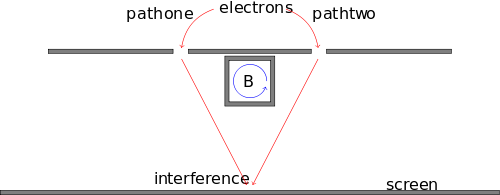
\includegraphics[width=300px]{aharanov-bohm.png}
    \caption{The setup of the solenoidal Aharonov-Bohm effect.}
    \label{fig:ab}
\end{figure}
The setup is as follows: consider an infinitely long cylindrical solenoid placed along the an axis. We now place a double-slitted wall in front of the solenoid and a detecting screen behind it, as shown in Fig.~(\ref{fig:ab}), and fire electrons at the wall.

It is simple to show (by Amp\`ere's Law) that the $E$ and $B$ fields are zero outside the solenoid, and so one would expect to see the usual double-slit interference pattern on the detecting screen. This is not the case, however! The mere presence of the solenoid yields a relative phase shift between electrons that go through different slits!

This phase difference actually stems from how electrons interact with the electromagnetic field -- there is a term in the Hamiltonian that is proportional to $\vec{A}\cdot\nabla$, i.e. the vector potential naturally in appears in the theory. Quantum mechanically, then, it is clear that the vector potential is a fundamental and physical dynamical variable. Indeed, the phase that each electron picks up is easily calculated (in the path integral formalism, modulo constants) to be
\[\phi=\int_\gamma A,\]
where $\gamma$ is a path taken by the electron. This expression is quite illuminating, as we can show that $A$ appears only in a gauge invariant manner. First note that the only physically observable quantity is the phase difference between the two electrons as measured by the shift in the interference pattern:
\[\Delta\phi=\int_{\gamma_1}A-\int_{\gamma_2}A\]
where $\gamma_1$ and $\gamma_2$ are the paths taken by the two
electrons, respectively.
If we now take $A'=A+d\theta$, the phase shift becomes
\begin{align*}
	\Delta\phi'&=\int_{\gamma_1}A'-\int_{\gamma_2}A'\\
    &=\int_{\gamma_1}A+d\theta-\int_{\gamma_2}A+d\theta\\
    &=\int_{\gamma_1}A-\int_{\gamma_2}A\\
    &=\Delta\phi.
\end{align*}
Here we have integrated out $d\theta$ to get $\theta(b)-\theta(a)$ from both integrals, where $a,b$ are the start and end points of $\gamma_1,\gamma_2$. Of course, since it appears in both integrals, the $\theta$ dependence simply cancels out. Hence we see that $A$ is truly a physical variable, and that it appears only in a gauge-invariant way.

But we've digressed a bit -- now that we understand that the connection $A$ is a fundamental quantity (at least in the case of electromagnetism), let us see how its gauge-invariance can lead to trouble. Recall the path-integral formalism of quantum mechanics: we compute probabilities by integrating $\exp(iS_{\text{SC}})$ over all possible paths a particle can take. In our case, we are not integrating over paths in spacetime, but instead over all possible gauge field configurations, $A$. This raises a subtle issue: if we truly integrate over all possible $A$'s, we'll be be summing over the infinitely many gauge-equivalent $A+d\theta$'s as well. But this is redundant! Physical information is stored only in the equivalence classes of $A$ since our observables are gauge-invariant. Indeed, $A'=A+d\theta$ should be treated as just \textit{being} $A$! This is the price of gauge symmetry; although it is often invaluable, one is forced to take great care when calculating quantum mechanical probabilities. Indeed, blindly integrating over all possible connections $A$ will mostly likely yield divergent results, as the infinitely many possible $d\theta$ additions will each contribute to the integral. Instead, one must integrate over some quotient space (sometimes called the ``moduli space''), having identified all gauge transformations of $A$ with $A$. In our case, we will have to integrate over $\Omega_1(M)/d\Omega_0(M)$, the space of all one-forms $A$ on $M$ modulo addition of exact forms. This space is often written as $\mathcal{A}/\mathcal{G}$, i.e. the space of connections modulo gauge transformations.

Note that here we have only been discussing quantizing our Chern-Simons theory via Feynman path integrals. Path integrals, by their very nature, are often rather mysterious beasts. One might inquire as to whether we can develop a canonical approach to quantization. The answer is actually yes. We will pursue this approach later, but it will require careful treatment of the phase space under the action of $\mathcal{G}$.

\subsection*{Wilson loops}

Now that we are a little more educated about gauge symmetry, it should be clear that observables are, essentially by definition, independent of gauge transformations, as gauge transformations are transformations that leave the physics unchanged. It is indeed one of the peculiarities of gauge theories that we introduce various symmetries only to demand in the end that everything physical be invariant under the action of said symmetry. Of course, as we have seen earlier in this course, the power of these symmetries in the context of generating charge, etc. cannot be understated.

We should ask, then: what are some invariants that appear in our $U(1)$ Chern-Simons theory? It is clear that any function of the curvature is a gauge invariant:
\begin{align*}
g(F')=g(dA')=g\big(d(A+d\theta)\big)=g(dA)=g(F)
\end{align*}
Unfortunately, in our $U(1)$ case, these functions would make poor observables since the equation of motion enforces $F=0$, i.e. any function of the curvature must be constant.

Are there any other ways to build gauge-invariant quantities? We have, in fact, seen one earlier! In the electromagnetic Aharonov-Bohm effect the relative phase that the electrons picked up was invariant under gauge transformations (or, if you will, well-defined on the moduli space). Using this as our motivation, we consider
\[W_{\gamma}[A]=\exp\left(i\oint_{\gamma} A\right),\]
which represents the change in phase of a single particle as it travels all the way around some loop $\gamma$. This quantity is often called a \textbf{Wilson loop} (by physicists) or a \textbf{holonomy} (by mathematicians) [\cite{baez}]. This observable intuitively measures an electron's change in phase experienced around some loop (for the more mathematically sophisticated, it returns, in some sense, information about how twisted our $U(1)$ principal bundle might be).

With Wilson loops in hand, let us discuss the basics of links and knots. 

\subsection*{Links and knots}
Knot theory is a large branch of mathematics that deals, roughly speaking, with classifying closed curves. In general, one can talk about knots without reference to an ambient space, but for our purposes we will consider knots embedded into the 3-manifold $M$ that our Chern-Simons theory is defined on. Thus, we formally define a \textbf{knot} as a submanifold of $M$ that is diffeomorphic to the circle, $S^1$ [\cite{baez}]. The simplest knot is the circle itself (often called the ``unknot''). Some more complicated knots can be seen in Fig.~(\ref{fig:knots}).

\begin{figure}[h]
	\centering
	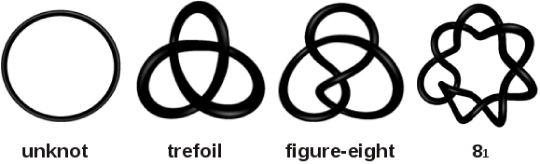
\includegraphics[width=200px]{unknot_trefoil.jpg}
    \caption{A few examples of knots}
    \label{fig:knots}
\end{figure}
We say that two knots are \textbf{equivalent} if there exists an \textbf{isotopy} between them, i.e. a map that continuously deforms one into the other, without ever causing different branches of the knot to intersect. Sometimes the equivalence of knots is counterintuitive: Fig.~(\ref{fig:isotopy}) shows how a very complicated knot can be deformed into the unknot. In this case, the isotopy between the initial knot and the unknot is hardly visible just by inspection. In fact, however hard it is to establish that two knots are equivalent, it is often even harder to determine that they are not. Indeed, how do we show that there exists no isotopy between the four knots presented in Fig.~(\ref{fig:knots})? Perhaps all knots are equivalent, and knot theory is just the overcomplicated study of the unknot under varoius disguises! We are therefore interested in finding a systematic procedure that can establish the equivalence of knots. The study of \textbf{knot invariants}, quantities left unchanged by isotopies, aims to solve precisely this problem. If two knots have different values for a knot invariant, then we can say for sure that they are not equivalent - in fact, this is how we can prove that the knots in Fig.~(\ref{fig:knots}) above are all distinct.
\begin{figure}[h]
	\centering
	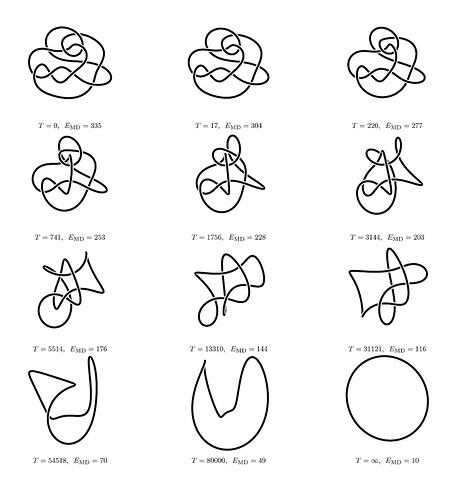
\includegraphics[width=200px]{unknot.jpg}
    \caption{Each of these knots is isotopic to the unknot!}
    \label{fig:isotopy}
\end{figure}
\\
In order to bring our discussion back to Chern-Simons theory, we need to be able to talk about \textbf{links}, or groups of knots. An example of this is presented in Fig.~(\ref{fig:ln}), where the curves $\gamma_1$ and $\gamma_2$ are knots in $M$, and their union is a link of two knots. Just as knots can be unexpectedly equivalent, two links that look different could be equivalent. A link in which two knots appear to be tied together can be, perhaps, deformed into a link in which they are separated. In order to distinguish between links, we use an invariant called \textbf{linking number}, which, roughly speaking, measures how many times one knot is wrapped around another. A linking number of 0, for example, corresponds to two disconnected knots; the link in Fig.~(\ref{fig:ln}) has linking number 2.

\begin{figure}[h]
	\centering
	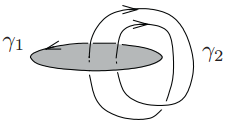
\includegraphics[width=100px]{knot_linking.png}
    \caption{Computing the linking number of a link \cite{infinite}.}
    \label{fig:ln}
\end{figure}
To make formal the definition of the linking number, we follow the procedure in \cite{infinite}. Notice that whenever $\gamma_2$ wraps around $\gamma_1$, it intersects transversally the surface $D_1$ bounded by $\gamma_1$ (the shaded area in Fig.~(\ref{fig:ln})). Therefore we define:
\begin{align*}
\text{lk}(\gamma_1, \gamma_2) = \int_{x\in D_1} \int_{y\in \gamma_2} \delta^{2,1} (x,y),
\end{align*}
where $\delta^{2,1}(x,y)$ is a 2-form that is nonzero only when $x\neq y$ (i.e. $\delta^{2,1} (x,y)$ is a form on $M\times M$, supported only on the diagonal of $M$). We can think about this as a differential form analog of the Dirac-delta distribution that cancels out contributions to the integral from unwanted regions on the manifold. The indices $2,1$ tell us that $\delta$ is a 2-form with respect to the variable $x$, which parametrizes a 2-dimensional surface, and a 1-form with respect to the variable $y$, which parametrizes a 1-dimensional curve. Therefore, the above integral will count the number of times that a point $x\in D_1$ is equal to a point $y\in \gamma_2$, which is exactly what we want from a linking number. For later use, we can rewrite this $\delta$-form as:
\begin{align}
\delta_{\gamma_2}(x) = \int_{y\in \gamma_2} \delta^{2,1}(x,y),
\label{eq:dgam}
\end{align}
where the subscript $\gamma_2$ reminds us that the form will be nonzero only when $x$ lies on the curve $\gamma_2$. Using similar notation, we can define an analogous form:
\begin{align}
\delta_{D_2}(x) = \int_{y\in D_2} \delta^{1,2}(x,y).
\label{eq:dD}
\end{align}
Now $y$ is constrained to the surface $D_2$, so this $\delta$ form is nonzero only when the free variable $x$ is on the surface $D_2$. If we assume that $D_2$ is simply connected, then we can relate $\delta_{\gamma_2}(x)$ and $\delta_{D_2}(x)$ by Stokes' theorem. Specifically:
\begin{align*}
\int_{x\in D_2} \delta_{D_2} (x) = \int_{x\in \partial D_2} d_x \delta_{D_2}(x) = \int_{x\in \gamma_2} \delta_{\gamma_2}(x),
\end{align*}
where the first equality is Stokes' theorem and the second simply says that $\gamma_2 = \partial D_2$. The index on $d_x$ is a reminder that we are taking an exterior derivative with respect to the variable $x$, not $y$. We conclude that $d_x \delta_{D_j}(x) = \delta_{\gamma_j} (x)$. Using this fact together with Eqs.~(\ref{eq:dgam}) and (\ref{eq:dD}) gives:
\begin{align*}
d_x (\delta^{1,2})(x,y) = \delta^{2,1} (x,y)
\end{align*}
Finally, note that in this formalism we can rewrite the linking number as:
\begin{align*}
\text{lk}(\gamma_1, \gamma_2) &= \int_{x\in D_1} \int_{y\in \gamma_2} \delta^{2,1} (x,y) \\
	&= \int_{x\in D_1} \delta_{\gamma_2}(x) \\
    &= \int_M \delta_{D_1} \wedge \delta_{\gamma_2}
\end{align*}
This calculus of $\delta$-forms will come in handy throughout the next section, where we develop the relationship between Chern-Simons theory and linking numbers.

\subsection*{The linking number from Wilson loops}

Quantum mechanics is, by and large, the study of the expectation values of observables. Physically, we cannot predict the outcome of any one measurement but only the average value over many measurements. We are therefore interested in computing the expectation value of the Wilson loop, $\langle W_{\gamma}[A]\rangle$ \cite{oldwine}.

In light of the delta-type forms used earlier in the theory of links, we rewrite the Wilson loop as:
\begin{align*}
W_\gamma[A]=\exp\left(i\oint_{\gamma} A\right) = \exp\left(i\int_{M} A\wedge \delta_{\gamma}\right)
\end{align*}
In words, what we have done is changed the domain of integration to all of $M$ instead of just the curve $\gamma$. To leave the integral unchanged, we multiply the integrand by a 2-form $\delta_{\gamma}$ which has support only on the loop $\gamma$.

Our ultimate goal is to connect the the expectation value of the Wilson loop to the linking number of some link, and thus, foreshadowing this result, we will integrate not only along the loop $\gamma$, but multiple such loops. Furthermore, we will
weight the contribution of each loop by some real $b_j$:
\begin{align*}
W[A]=\prod_j \exp\left(i b_j \int_{M} A\wedge \delta_{\gamma_j}\right) =\exp\left(i\int_{M} A\wedge (\sum_j b_j \delta_{\gamma_i})\right)
\end{align*}
The reason we wish to generalize the Wilson loop in this way is to recover a linking number of a link with multiple components, instead of the self-linking of just $\gamma$ (which in fact often turns out to be divergent without some kind of regularization)\cite{infinite}. Of course, with this generalization we have distanced ourselves from the physical example of the Aharonov-Bohm effect. While this is unfortunate, it is a necessary evil.

Now, applying a well-known result from the theory of path integrals, we find that the expectation value is:
\begin{align*}
\langle W[A] \rangle&=\frac{\int DA \; W[A]\; \exp\left(iS_{CS}\right)}{\int DA \;\exp\left(iS_{CS}\right)}\\
&=\frac{\int DA \; \exp\left(i\int_{M} A\wedge (\sum_j b_j \delta_{\gamma_i})\right)\; \exp\left(i\int_M A\wedge dA\right)}{\int DA \;\exp\left(i\int_M A\wedge dA\right) }
\end{align*}
Before we carry out the computation, it is important to understand our path integral's domain of integration. We typically interpret the integration measure $DA$ as integrating over the space $\Omega_1(M)$ of all 1-forms $A$ over the manifold $M$. However, if we attempt to do this, gauge invariance will cause the integral to diverge, as we noted earlier; the integrand is constant when $A$ is gauge-transformed to $A+d\theta$, so integrating over this degree of freedom yields a divergent result. To avoid this, we interpret the path integral as running over equivalence classes $[A] = [A+d\theta]$ in the quotient space $\Omega_1(M)/d\Omega_0(M)$.

Note that the Chern-Simons action is quadratic in $A$, while the Wilson loop is linear. We can therefore complete the square in the exponent in order to obtain a Gaussian integral in the numerator of the expectation value. Next, using the usual Gaussian integral tricks (c.f. \cite{infinite}), we obtain:
\begin{align}
\langle W[A] \rangle &= \exp\left(\frac{1}{2} \int_M A_0 \wedge (\sum_j b_j \delta_{\gamma_i}) \right)
\end{align}
where $A_0$ solves $dA + (\sum_j b_j \delta_{\gamma_i}) = 0$. Now we can use the calculus of $\delta$-forms derived in the previous section to rewrite the result as:
\begin{align*}
\langle W[A] \rangle &= \text{exp} \left\{ \frac{1}{2} \int_{x\in M} A_0(x)\wedge \sum_j b_j \int_{y\in \gamma_j} \delta^{2,1} (x,y)     \right\} \\
	&= \exp\left\{\frac{1}{2} \int_{x\in M} A_0(x) \wedge \sum_j b_j \int_{y\in D_j} d_x \delta^{1,2} (x,y)\right\}
\end{align*}
We integrate by parts in order to move the exterior derivative on $A_0$, picking up a minus sign in the process:
\begin{align*}
\langle W[A] \rangle &= \text{exp} \left\{ \frac{1}{2} \int_{x\in M} (-dA_0) \wedge \sum_j b_j \int_{y\in D_j} \delta^{1,2} (x,y)  \right\}
\end{align*}
But recall that, by definition, $-dA_0 = \sum_k b_k \delta_{\gamma_k}$, so:
\begin{align*}
\langle W[A] \rangle &= \text{exp} \left\{  \frac{1}{2} \int_{x\in M} \big( \sum_k b_k \delta_{\gamma_k} (x) \big) \wedge \big( \sum_j b_j \delta_{D_j} (x) \big) \right\} \\
	&= \text{exp} \left\{  \frac{1}{2} \sum_{j,k} b_k b_j \int_{x\in M} \delta_{\gamma_k}(x) \wedge  \delta_{D_j} (x) \right\} \\
    &= \text{exp} \left\{  \frac{1}{2} \sum_{j,k} b_k b_j \text{lk}(\gamma_k, \gamma_j) \right\}
\end{align*}
This is a truly remarkable result! We embarked on this calculation in pursuit of the expectation value for arbitrary, multi-component, Wilson loops in our Chern-Simons theory on $M$, and we have recovered precisely a sum of the pairwise linking numbers of our loops!
In other words, computing the average value of a quantum mechanical observable has given us topological information about embeddings of circles into $M$ -- truly the name \textit{topological} quantum field theory is well-deserved. Note, incidentally, that the sum includes the self-linking numbers of each component of the link (each individual Wilson loop). Additionally, the factor of one-half automatically accounts for double-counting of the pairwise linkings.


\subsection*{Further exploration}
The computation that we have carried out turns out to be a simplified version of a much more powerful relation between Chern-Simons theory and knot invariants. If we consider non-abelian Chern-Simons theories, i.e. use $SU(2)$ or $SU(3)$ instead of $U(1)$ as a gauge group, we get a vastly more complicated theory, which yields more interesting invariants. To get a feel for what happens in the non-Abelian case, note that the general form of the Chern-Simons action is:
\begin{align*}
S_{\text{CS}} = \int_M \text{tr}\left(A\wedge dA + \frac{2}{3}A\wedge A \wedge A\right).
\end{align*}
Here $A$ is no longer a real-valued form, but instead takes on values in the Lie algebra of the gauge group. In particular, we have to take the trace of the resulting operator in order to obtain a real-valued Lagrangian. The wedge product we use here is a good measure of how much more complicated the theory is. It is no longer the usual antisymmetric wedge product defined on real-valued forms, which would vanish when we feed it different copies of the same form $A$. Another problem is that the action is no longer quadratic in $A$, due to the presence of the cubic term. This means that the expectation value of the Wilson loop, computed easily in the abelian case via the usual Gaussian integral tricks, can no longer be computed in closed form. We must turn instead to perturbation theory, a long, tedious, and inexact procedure. On the bright side, it is currently thought that the correction to the expectation value to any order is a knot invariant in and of itself \cite{oldwine}! To first order, the result is the linking number that we computed above; the following orders are called the Vassiliev numbers. Vassiliev conjectured that the class of invariants obtained from all orders can completely classify all knots - in other words, any two knots that have the same invariants obtained from Chern-Simons theory are equivalent! This conjecture has not been proved so far, but it has been shown that large classes of knots can be distinguished using Vassiliev numbers. Consequently it appears that the  2+1-dimensional Chern-Simons topological quantum field theory, of all things, may be the object of fundamental importance in the field of knot theory.

\subsection*{Acknowledgements}

We would like to thank Professor Peter Woit for providing us with the opportunity to learn and present these ideas, as well as imparting to us innumerable physical and mathematical insights.  


\begin{thebibliography}{5}

\bibitem{oldwine}
	Am. J. Phys. \textbf{66}, 1060 (1998); doi: 10.1119/1.19046
\bibitem{infinite}
	Boris Khesin and Robert Wendt, \emph{The Geometry of Infinite-Dimensional Groups}.
    Springer Berlin Heidelberg, 2009.
\bibitem{baez}
	John Baez and Javier P. Munian, \emph{Gauge Fields, Knots and Gravity}.
    World Scientific Publishing Company, Incorporated, 1994.

\end{thebibliography}

\end{document}



% figure 1: http://upload.wikimedia.org/wikipedia/commons/2/2f/Aharonov-Bohm_effect.svg

% figure 2: http://ej.iop.org/images/1742-5468/2012/11/P11022/Full/jstat452025f1_online.jpg

% figure 3: http://farm3.static.flickr.com/2151/2091741335_9823fb3b5b.jpg

% figure 4: Boris Khesin and Robert Wendt, \emph{The Geometry of Infinite-Dimensional Groups}


% [\cite{baez}]











































